\begin{figure}[H]
    \centering
    \begin{mdframed}
        \centering
        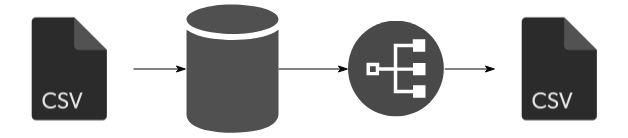
\includegraphics[scale=0.35]{./resources/figures/analysis.png}
    \end{mdframed}
    \caption[Analysis Workflow]{\textbf{Figure \ref{analysis}: Workflow to perform an analysis.} The analysis process represented as a simple pipeline. First nETL extracts data from CSV files and loads that into a CouchDB database via the CouchDB server API. This file consists of a B+tree organized by the \_id field of each document created as a UUID on document write by CouchDB to guarantee uniqueness of every document. From the database file an index is created, also structured as a B+tree but organized by a key as a specified in the Map Function. This allows for sorted output according to a users requirements. A List function is used to retrieve the contents of the view, transform those contents into tabular (CSV) form. The result of calling the List function is a downloaded CSV file. The List function address (API) is of the form \texttt{http(s)://<host>:<port>/<db>/\_design/<doc>/\_list/<fn>/<view>?<params>}}
    \label{analysis}
\end{figure}